\chapter{Desarrollo}

\section{Evalúe la exactitud de su fotocolorímetro con muestras reales coloreadas (colorante diluido) al menos para 4 absorbancias: 0, 0.5, 1 y 1.5.Cuyo valor de referencia sea el medido con un colorímetro Neulog para el mismo color.}

Para la elaboración del fotocolorimetro se tuvieron en cuenta varios aspectos previos al diseño circuito en función al microcontrolador ubicando como parte fundamental de su desarrollo la estructura para lo cual se hizo un modelado en 3D adaptando los circuitos de forma precisa en cada caso, seguidamente en función a los niveles de corriente para cada color en el microcontrolador se vario la intensidad del voltaje de salida en sus pines PWM y finalmente se adapto la lectura de la absorbancia mediante el pin analógico mediante un divisor de tensión con un LDR.

Cada parte del proceso fue de vital importancia para aproximar la exactitud de las mediciones a obtenidas con fotocolorimetro Neulog y cuya tabla de resultados para los valores propuestos se muestran en  \ref{tab:med-absorbancia}

\begin{table}[]
	\centering
	\begin{tabular}{|c|c|c|}
		\hline
		\textbf{\begin{tabular}[c]{@{}c@{}}Abs\\ Medido\end{tabular}} & \textbf{\begin{tabular}[c]{@{}c@{}}Abs\\ Neulog\end{tabular}} & \textbf{Error} \\ \hline
		0.3                                                           & 0                                                             &                \\ \hline
		0.45                                                          & 0.5                                                           & 10             \\ \hline
		0.89                                                          & 1                                                             & 11             \\ \hline
		1.37                                                          & 1.5                                                           & 8.66666667     \\ \hline
	\end{tabular}
	\caption{Comparación de absorbancia Neulog - Fotocolorimetro implementado}
	\label{tab:med-absorbancia}
\end{table}

Y de la cual se puede enfatizar cierta exactitud por comparación del fotocolorimetro diseñado y el disponible para el laboratorio reafirmando según la experiencia la ley de Beer Lambert.

\section{Presente el código de su fotocolorímetro y explique su funcionamiento mediante un diagrama de flujo.}

\begin{figure}[h]
	\centering
	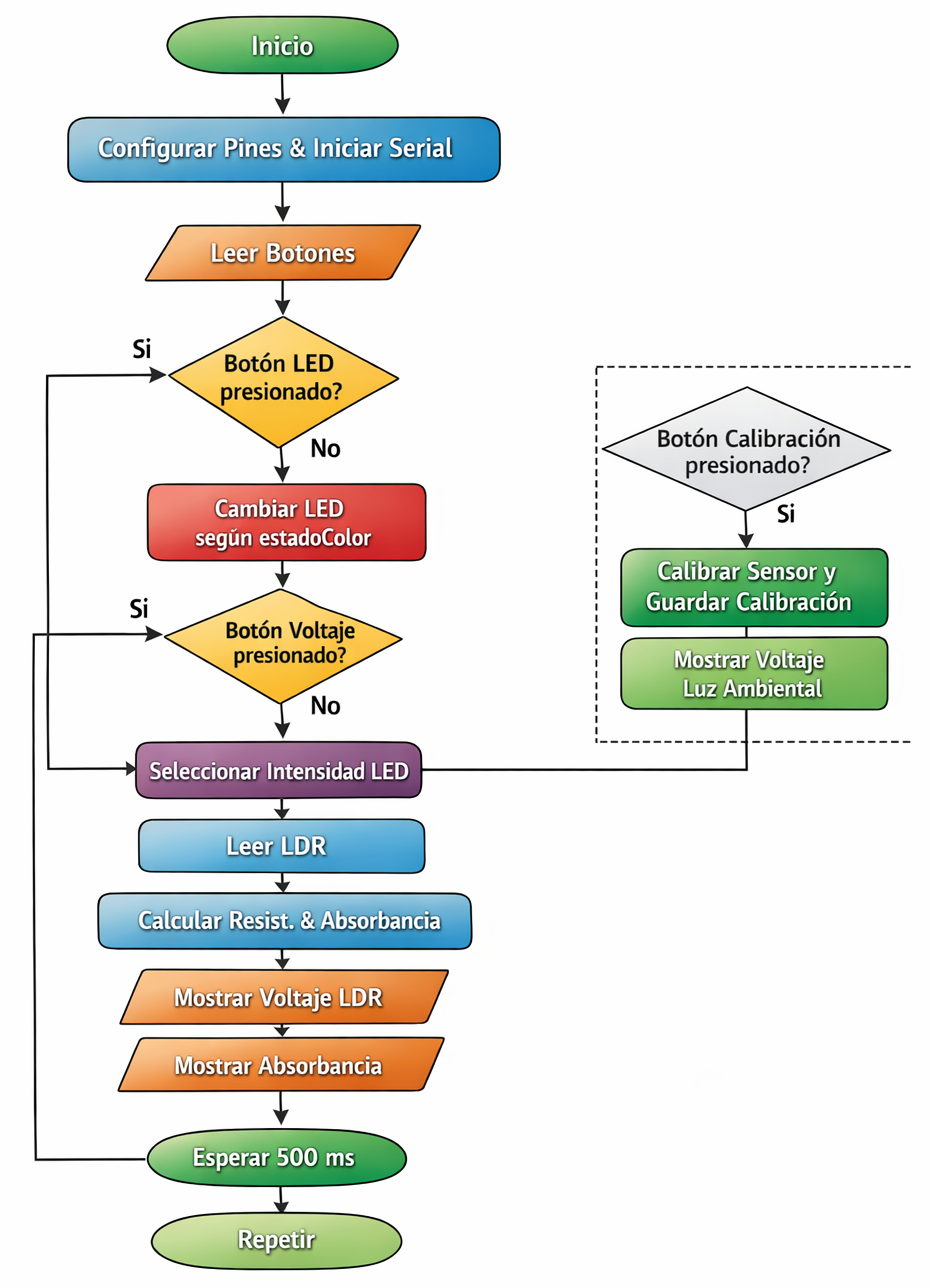
\includegraphics[width=0.7\linewidth]{media/diagrama-flujo}
	\caption{Diagrama de flujo del código Arduino - fotocolorimetro}
	\label{fig:diagrama-flujo}
\end{figure}

El diagrama de flujo \ref{fig:diagrama-flujo} describe el funcionamiento del fotocolorímetro basado en Arduino que utiliza un led RGB y un sensor LDR para medir la absorbancia de una muestra. El proceso inicia con la configuración de los pines de entrada y salida del microcontrolador y la inicialización de la comunicación serial. Luego, dentro del ciclo principal del programa, el sistema lee continuamente el estado de los botones que permite cambiar el color del LED activo (rojo, verde o azul) y con otro modificar la intensidad del LED, alternando entre diferentes niveles de voltaje predefinidos. Dependiendo del estado seleccionado, el sistema enciende el LED correspondiente y apaga los demás, asegurando que solo un color ilumine la muestra en cada momento.

Posteriormente, el sistema realiza la lectura analógica del sensor LDR, el cual detecta la cantidad de luz que atraviesa la muestra iluminada por el LED seleccionado. A partir de esta lectura se calcula el voltaje del sensor, la resistencia equivalente del LDR y finalmente la absorbancia, utilizando una relación logarítmica basada en el voltaje medido. Estos valores se envían al monitor serial para su visualización y análisis. Después de mostrar los resultados, el sistema espera un breve intervalo de tiempo (500 ms) y repite el ciclo, permitiendo realizar mediciones continuas mientras el usuario puede cambiar el color del LED o la intensidad de iluminación según sea necesario.



